\documentclass[11pt]{scrartcl}

\usepackage{graphicx}

\title{Arbeitsübersicht}
\author{Kristina Thieme}
\date{\today{}}

\begin{document}
\maketitle

\section{Datensatz}

In dem Datensatz der Seagate Expansion Festplatte sind 960GB Dateien. Diese sind in 13 Ordnern aufgeteilt, die in dem Zeitraum vom
15.07.2022 bis 29.08.2022 aufgenommen wurden. Die Bilder wurden meist in der Zeit von 6:00 morgens bis 23:00 abends aufgenommen. 
Um den größten Ordner von ca 300GB einzulesen zur Verarbeitung, hat es ca eine halbe Stunde bis 40 Minuten gedauert.


\subsection{Filter Algorithmus}

Die Bilder in den Ordnern müssen gefiltert werden, da der Großteil des Datensatzes keine Objekte von Interesse behinhaltet. 
Ich habe mit Python und der Library OpenCV einen Algorithmus geschrieben, der die Bilder der einzelnen Ordner einliest und jeweils 
ein Bild mit dem nächsten vergleicht. Ist der Unterschied der beiden Bilder groß genug, wird das erste der Bilder in einen neuen
Ordner abgespeichert. Es werden immer zwei nebeneinander liegende Bilder verglichen, da dort die Veränderungen die nicht von Interesse sind,
wie zum Beispiel der Sonnenstand oder Wind, zum größten Teil nicht viel zum Differenzwert beitragen, da der Unterschied zeitlich klein
genug ist. 

\subsection{Outcome}

Im Ordner vom 03.08.2022 wurde mehr als die Hälfte an Bildern weiter abgespeichert, da sich dort ein noch nicht zugeordnetes Insekt
bewegt. Die Bilder können dennoch hilfreich sein, da sie in das Cluster "Insekt, aber keine Schwebefliege" fallen. Der Großteil der Bilder,
auf denen Schwebefliegen zu erkennen sind, sind in den Ordnern vom 16.07.2022, 17.07.2022 und 18.07.2022. Auf den gefilterten Bildern vom 
23.08.2022, 24.08.2022, 26.08.2022 und 29.08.2022 wurden vorwiegend Bilder gefilert, auf denen ein Stück Corna-Test Müll sich im 
Wind bewegt hat. Dennoch sind insgesamt 2,41GB an Bildern von Schwebfliegen zusammen gekommen. Zusätzlich noch 8,62GB mit Insekten, die keine sind.

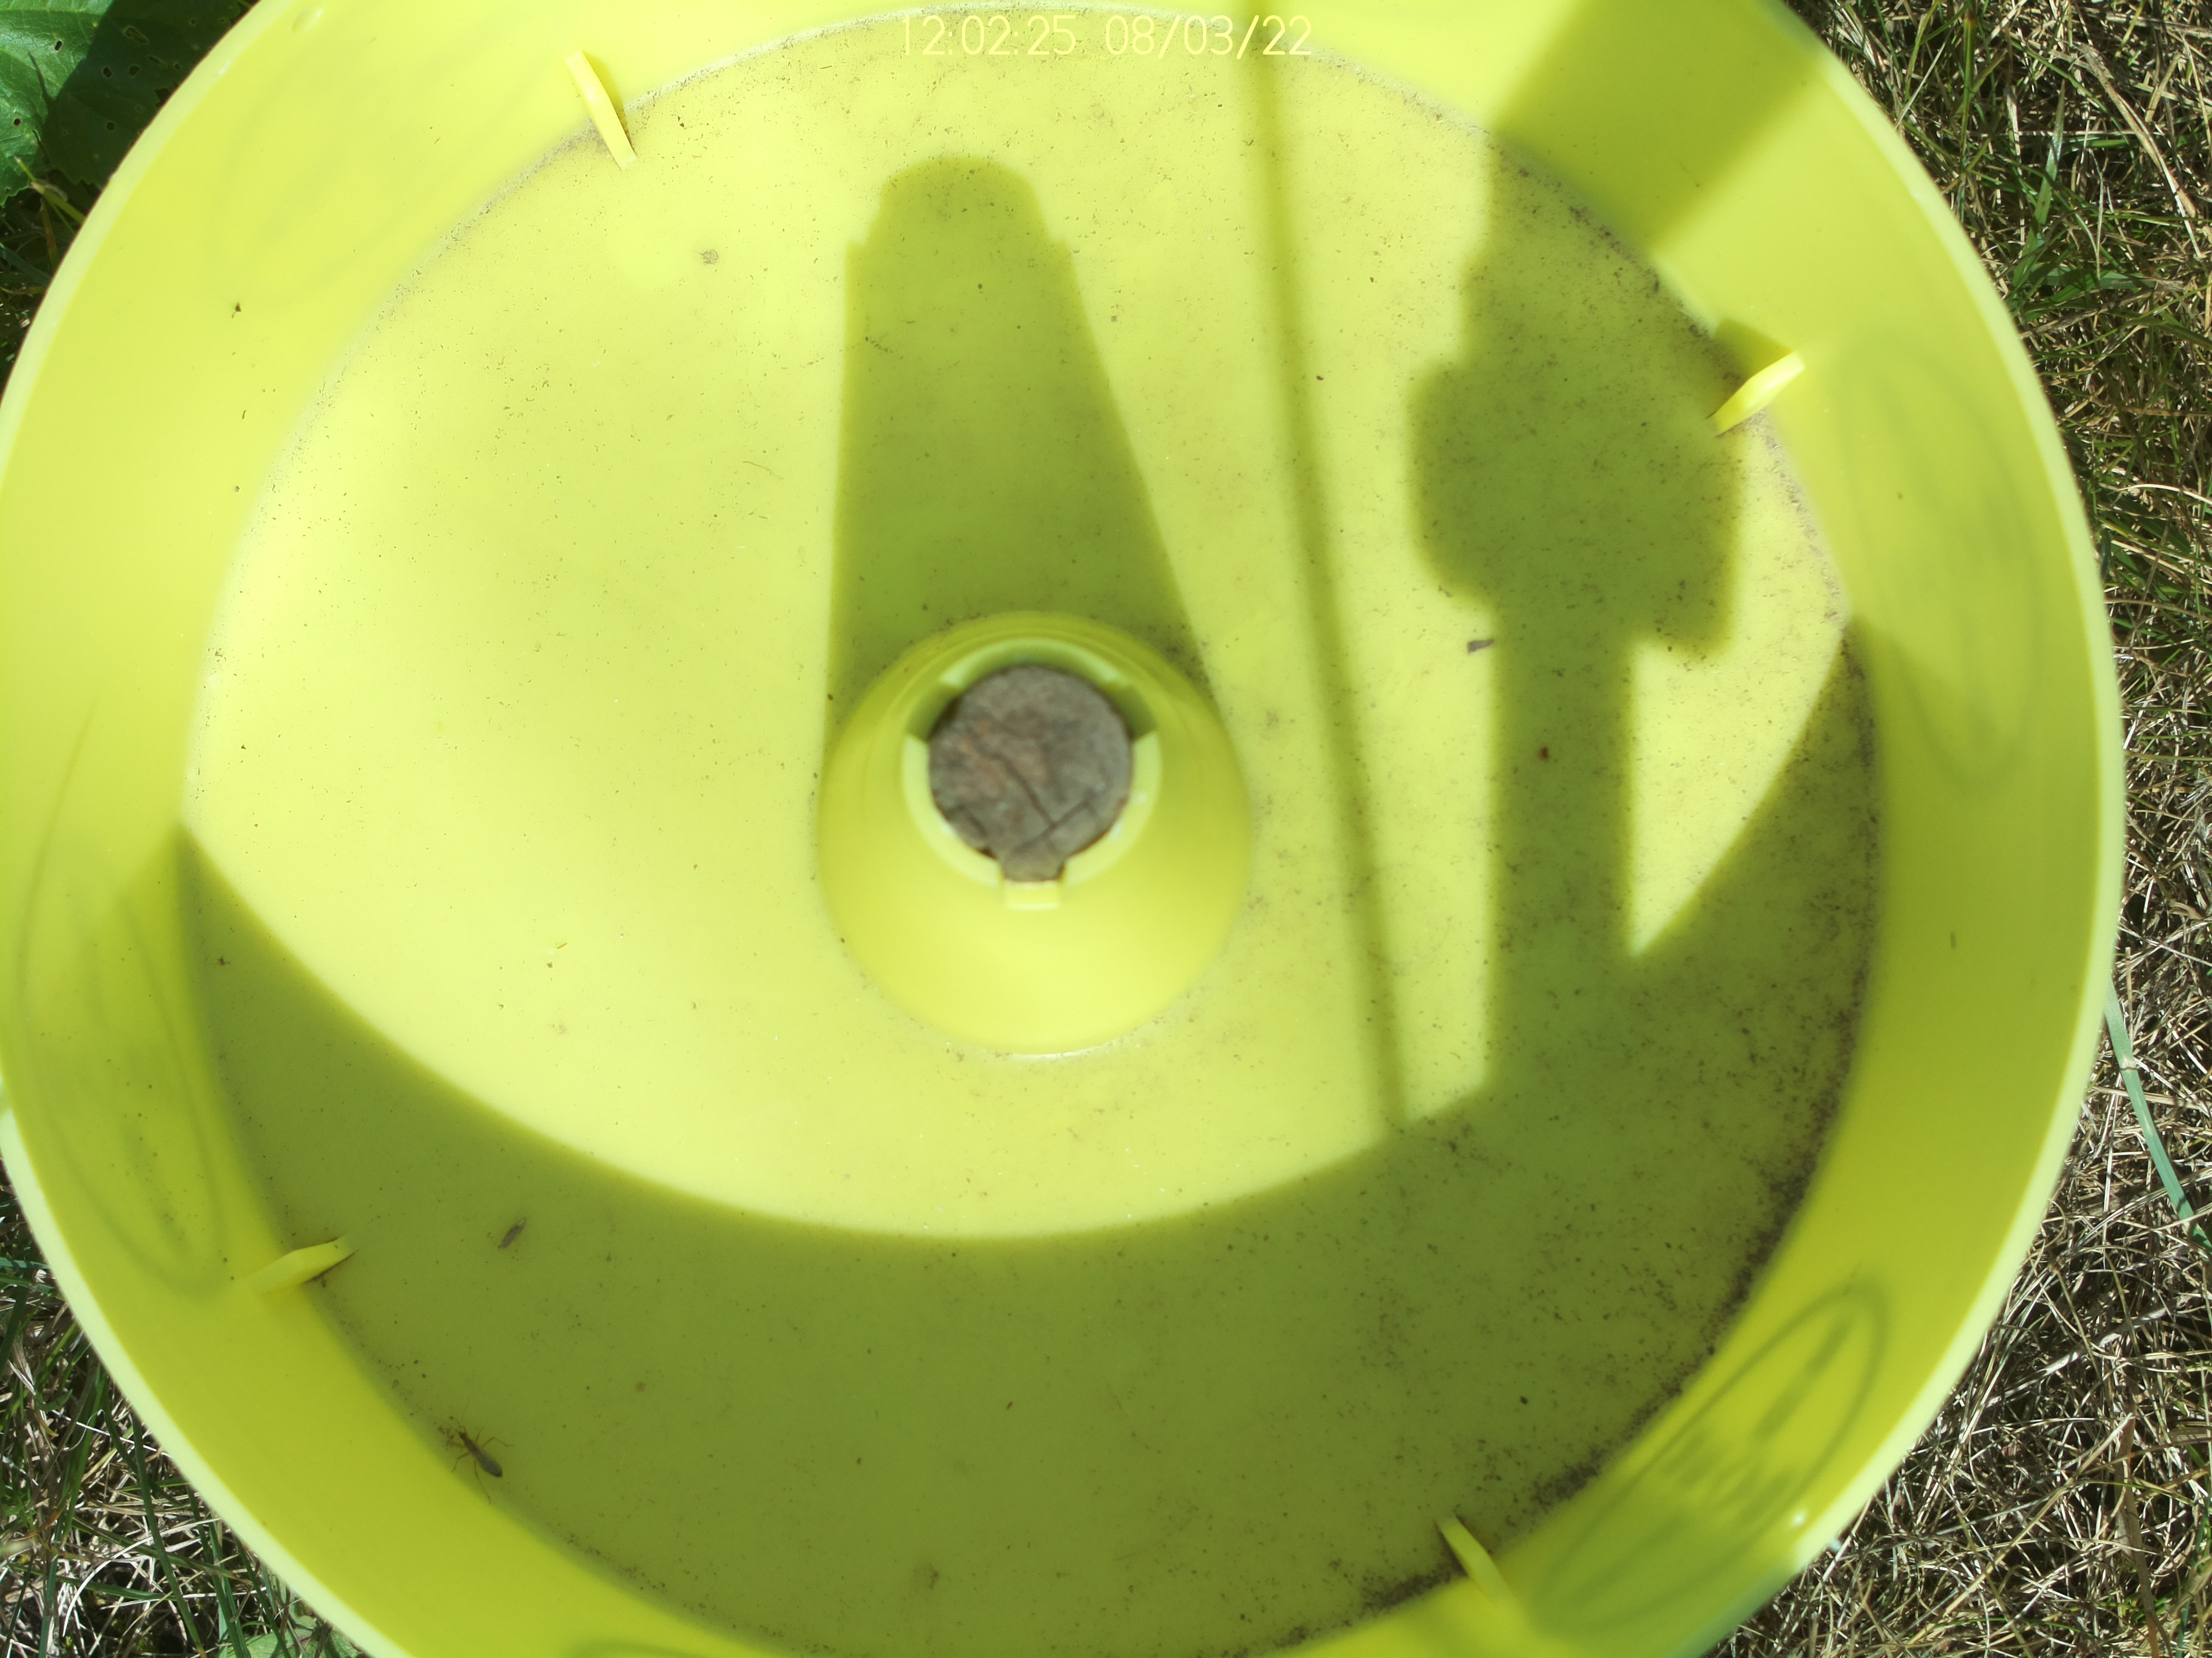
\includegraphics[width=0.6\textwidth]{diff144}

Das obrige Bild zeigt ein Insekt, dass nicht zu dem Cluster "Schwebefliege" gehört\\

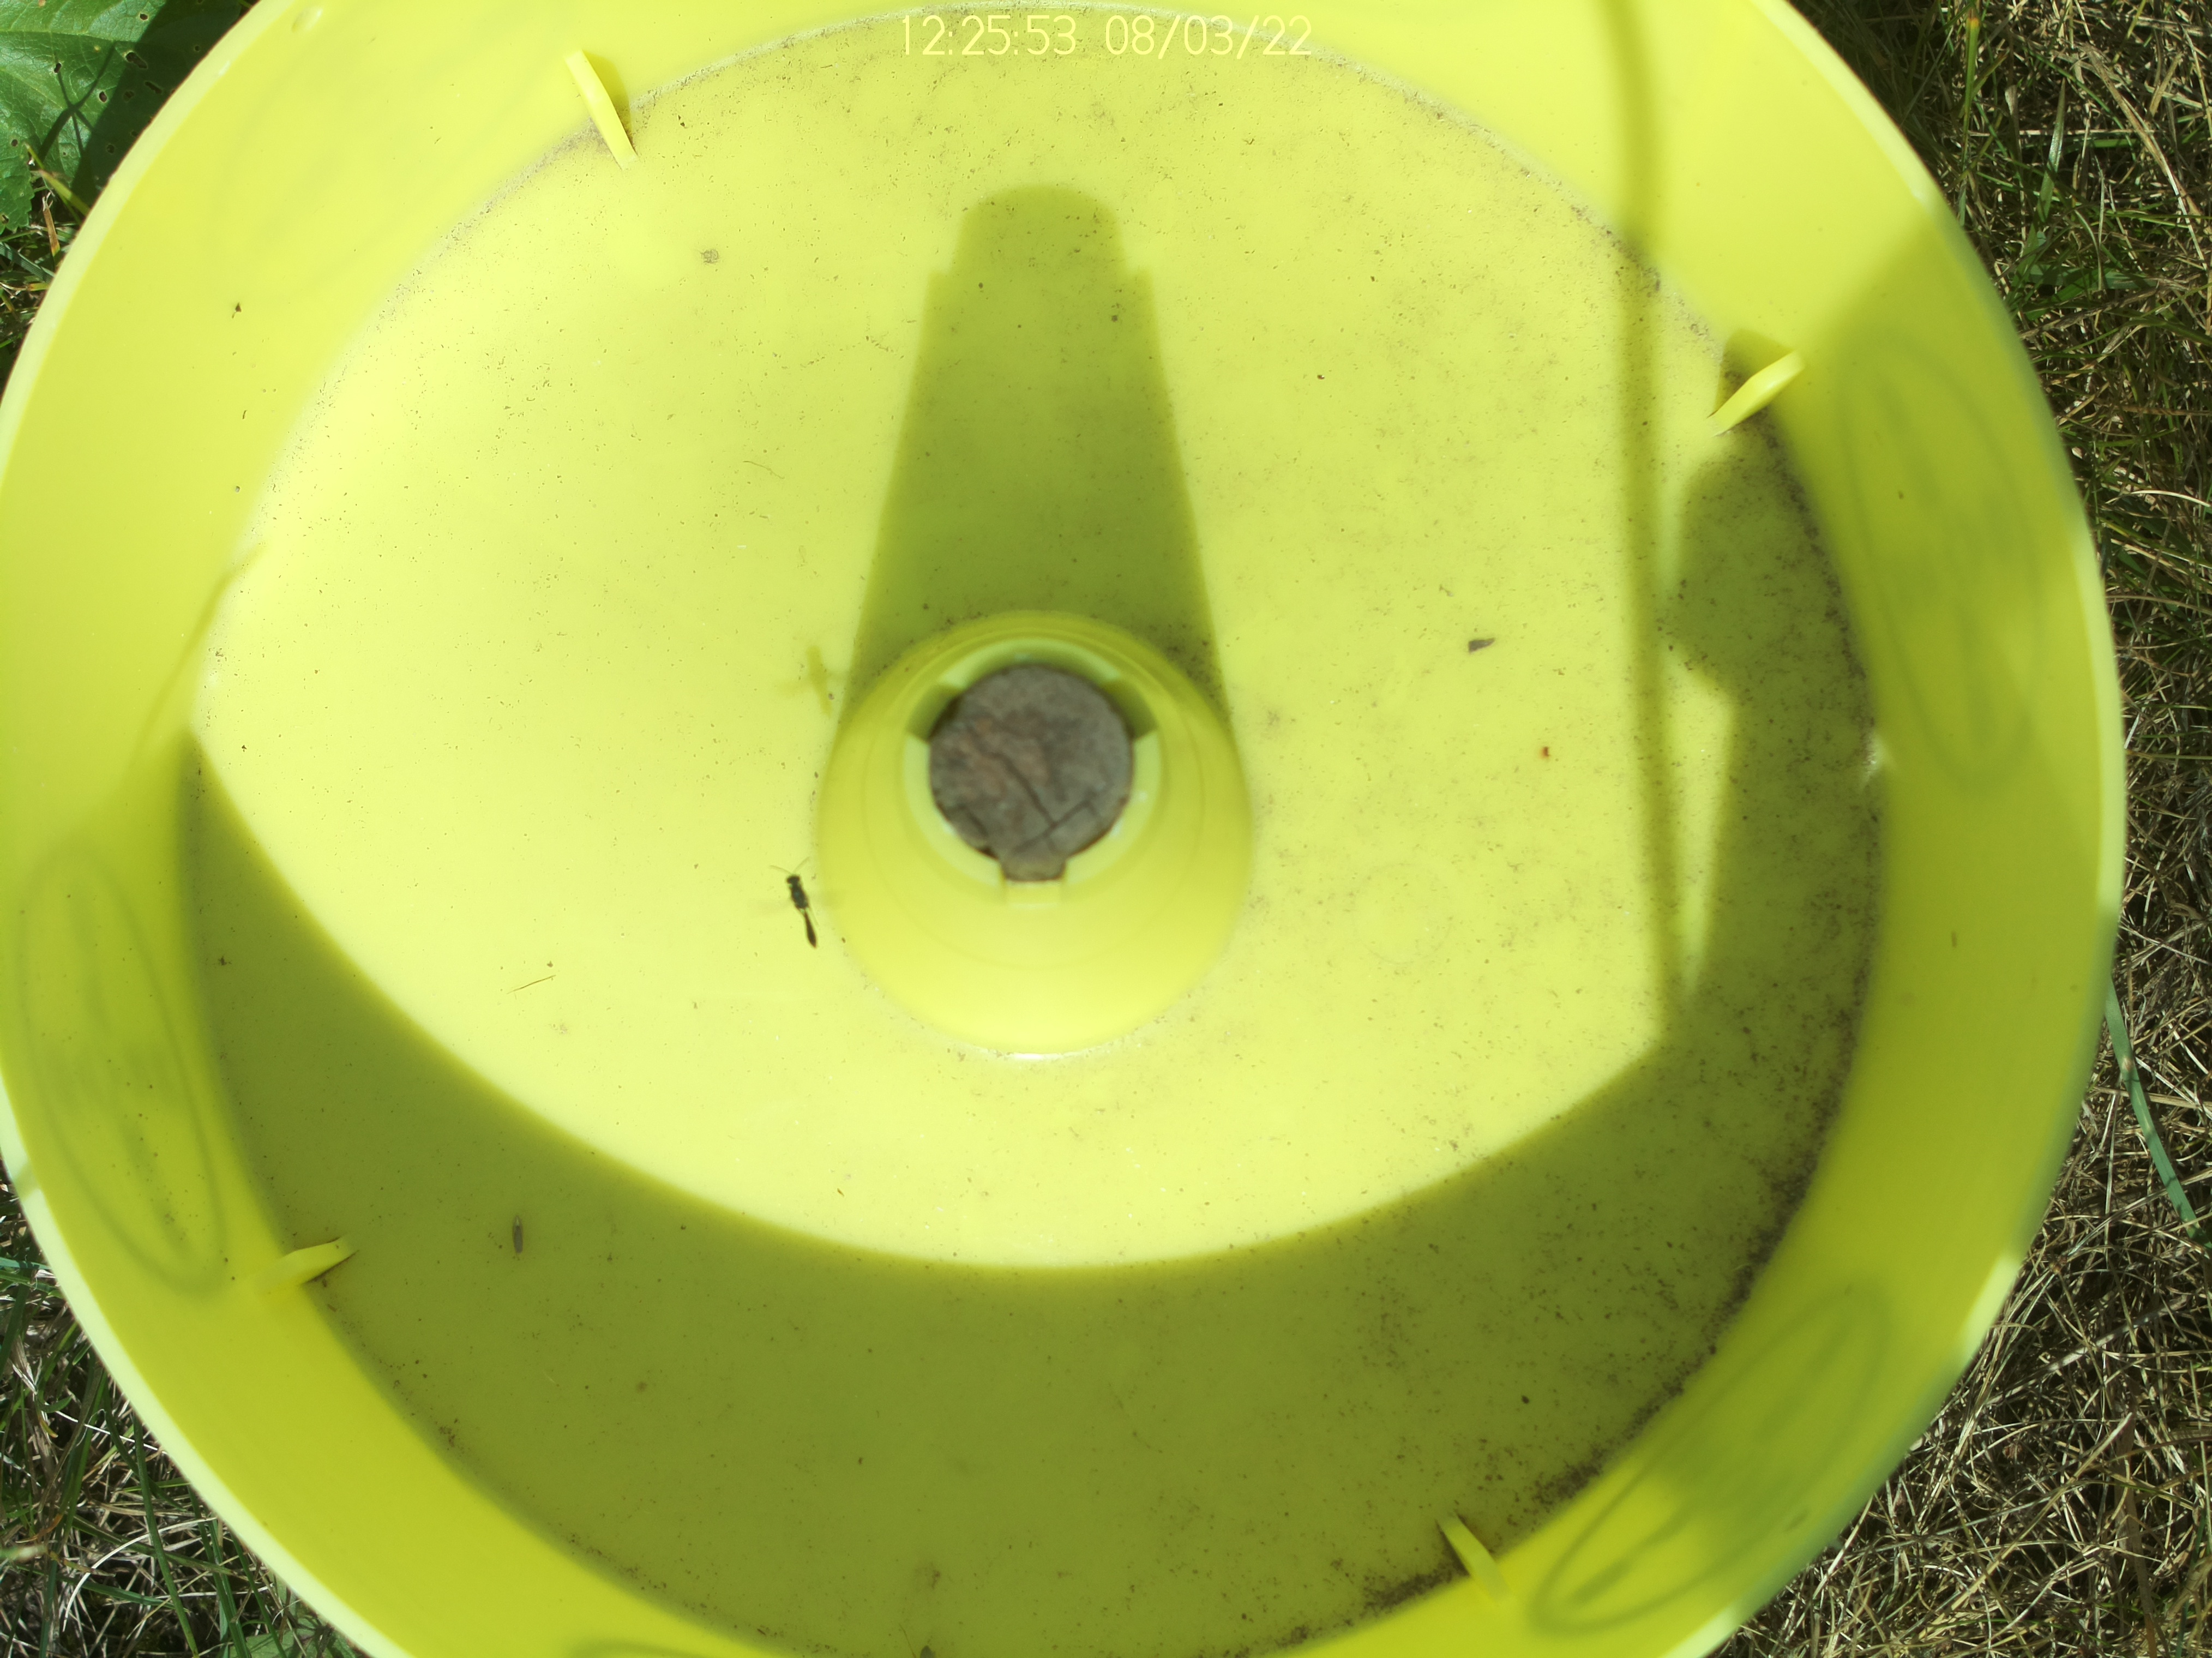
\includegraphics[width=0.6\textwidth]{diff1552}

Das obrige Bild zeigt eine Schwebefliege


\subsection{Clustering}

Es gibt mehrere Unterschiede die zwischen den Bildern zu ziehen sind. Nachdem man zwischen "Schwebefliege" und "nicht Schwebefliege" 
unterscheidet, kann man das Cluster "Schwebfliege" weiter aufteilen. Die Bilder sind aufteilbar in folgende Cluster: "Kleine Schwebefliege",
"Mittelgroße Schwebefliege", "Große Schwebefliege" und wenn nötig "Tote Schwebefliege" Im Folgenden weiter Beispielbilder zu den 
eben genannten Clustern.\\

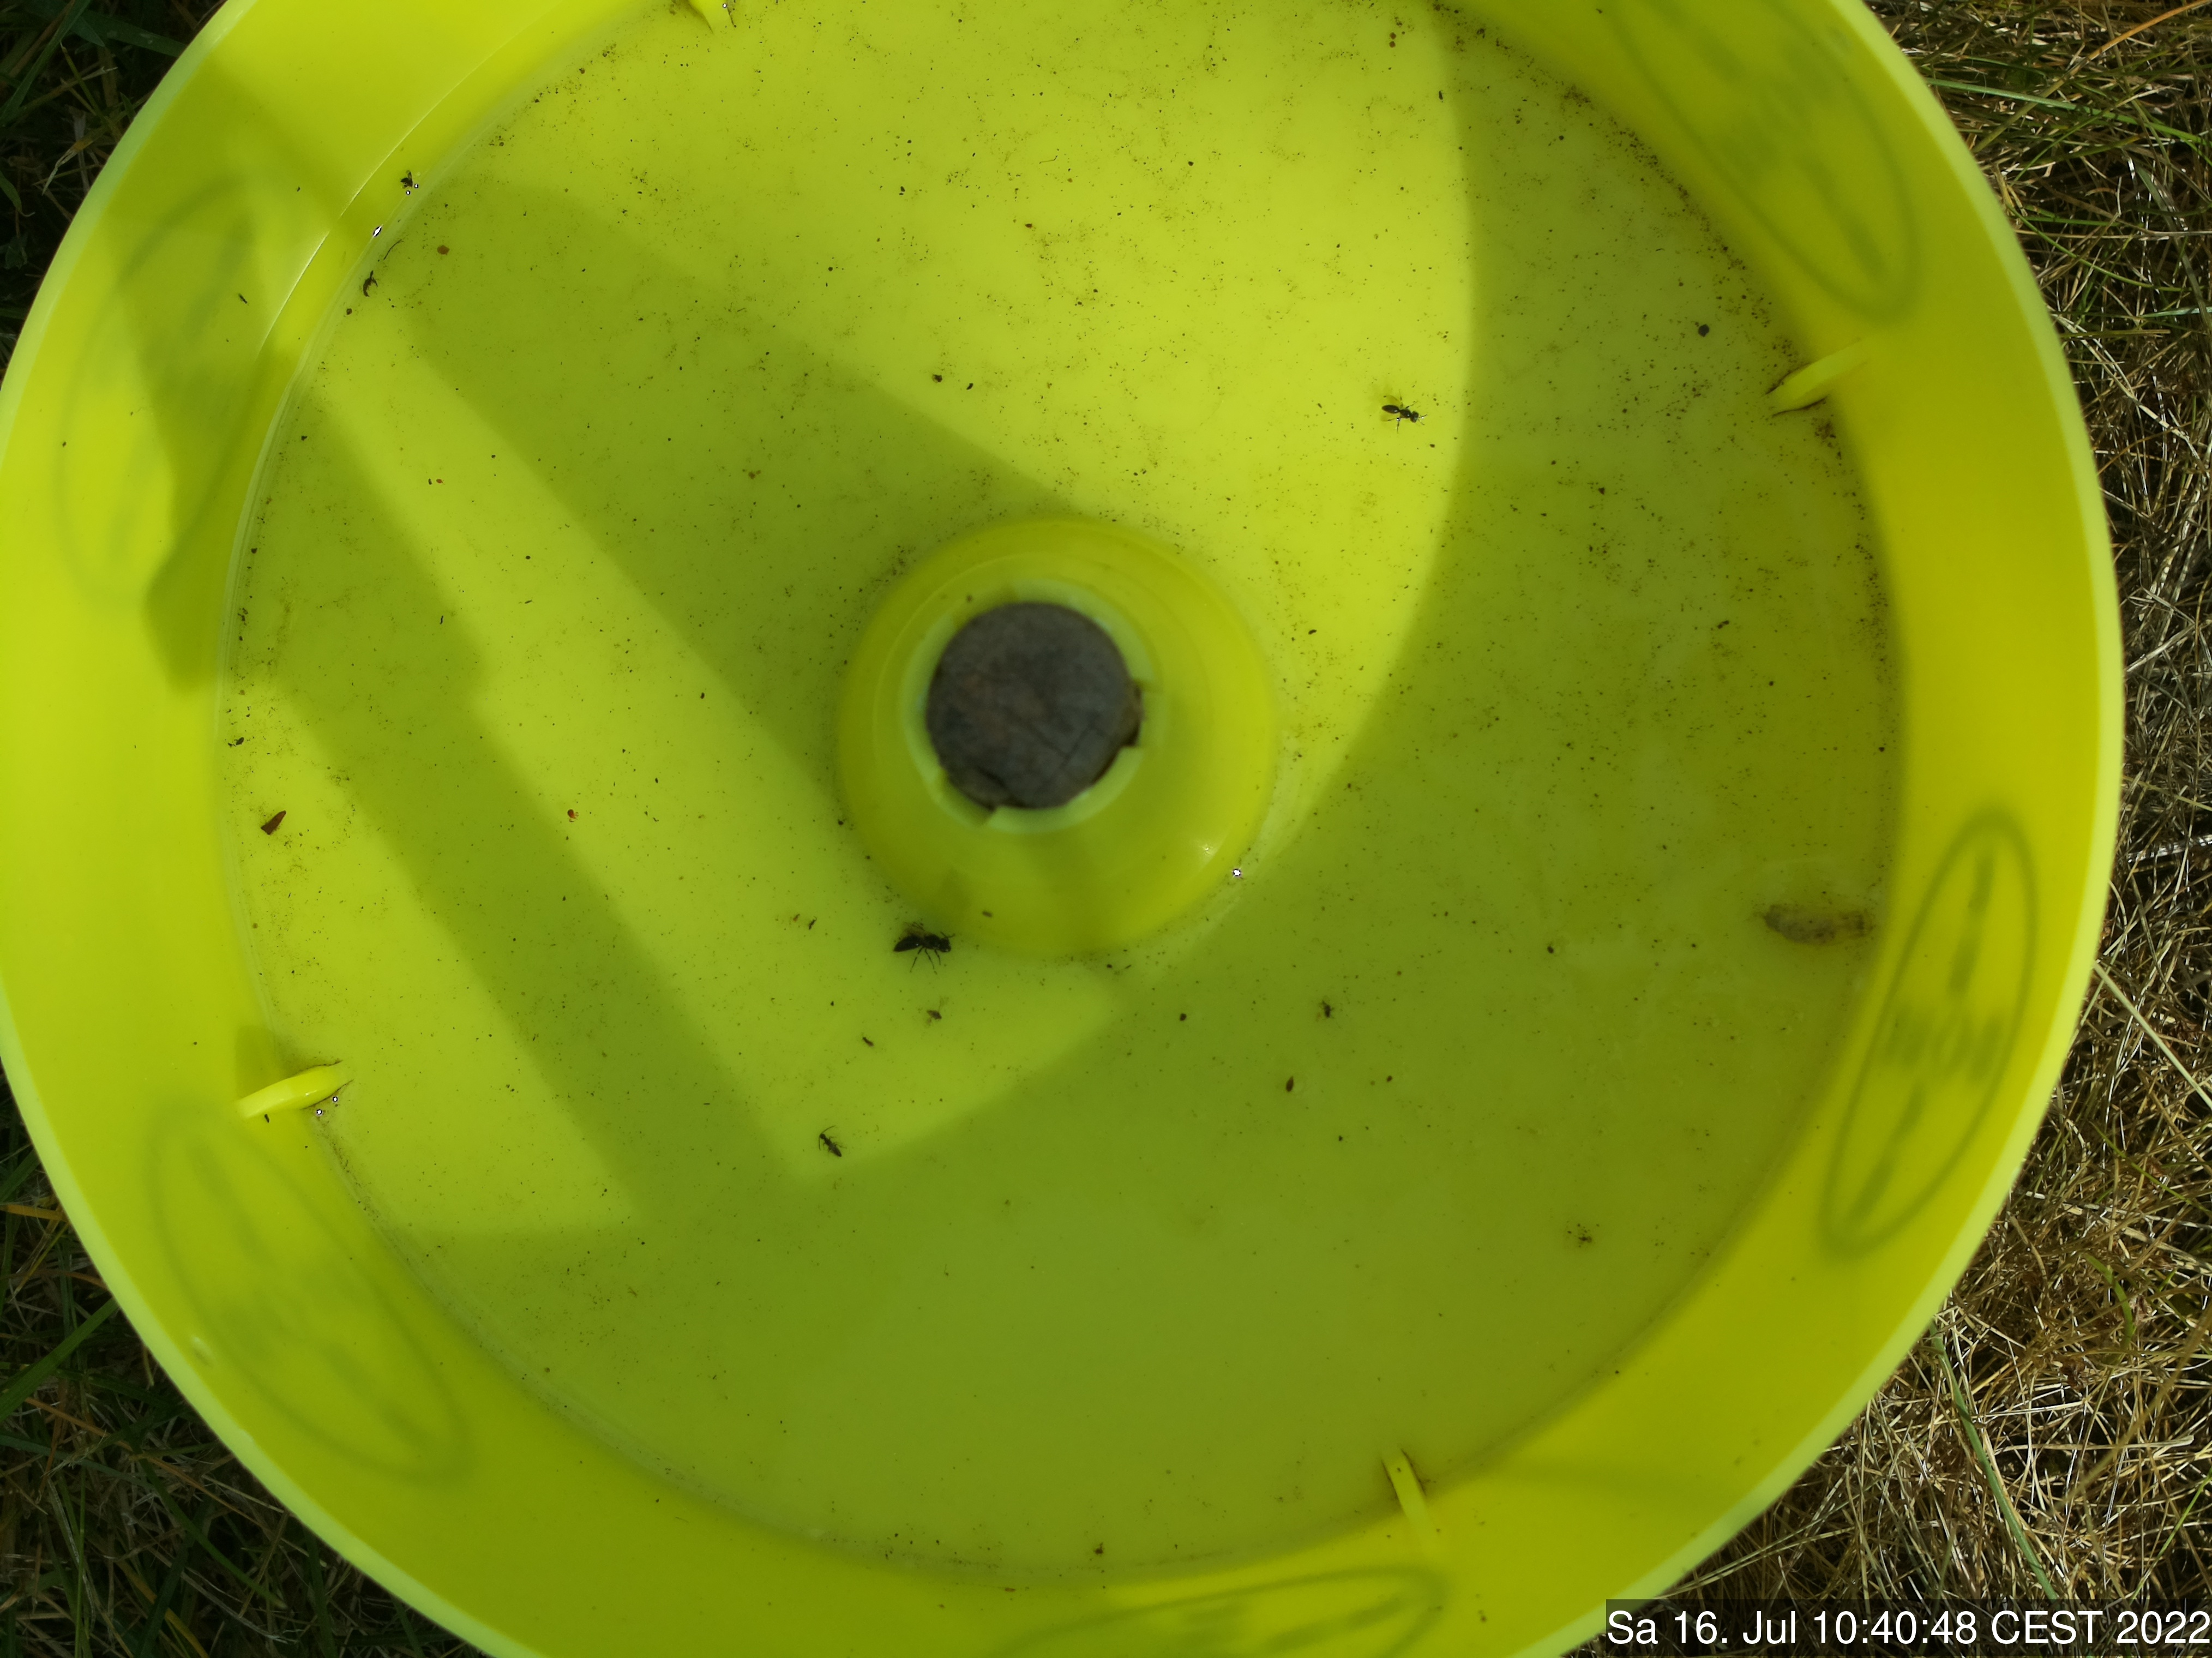
\includegraphics[width=0.5\textwidth]{diff4079}

Das obrige Bild zeigt eine kleine Schwebefliege\\

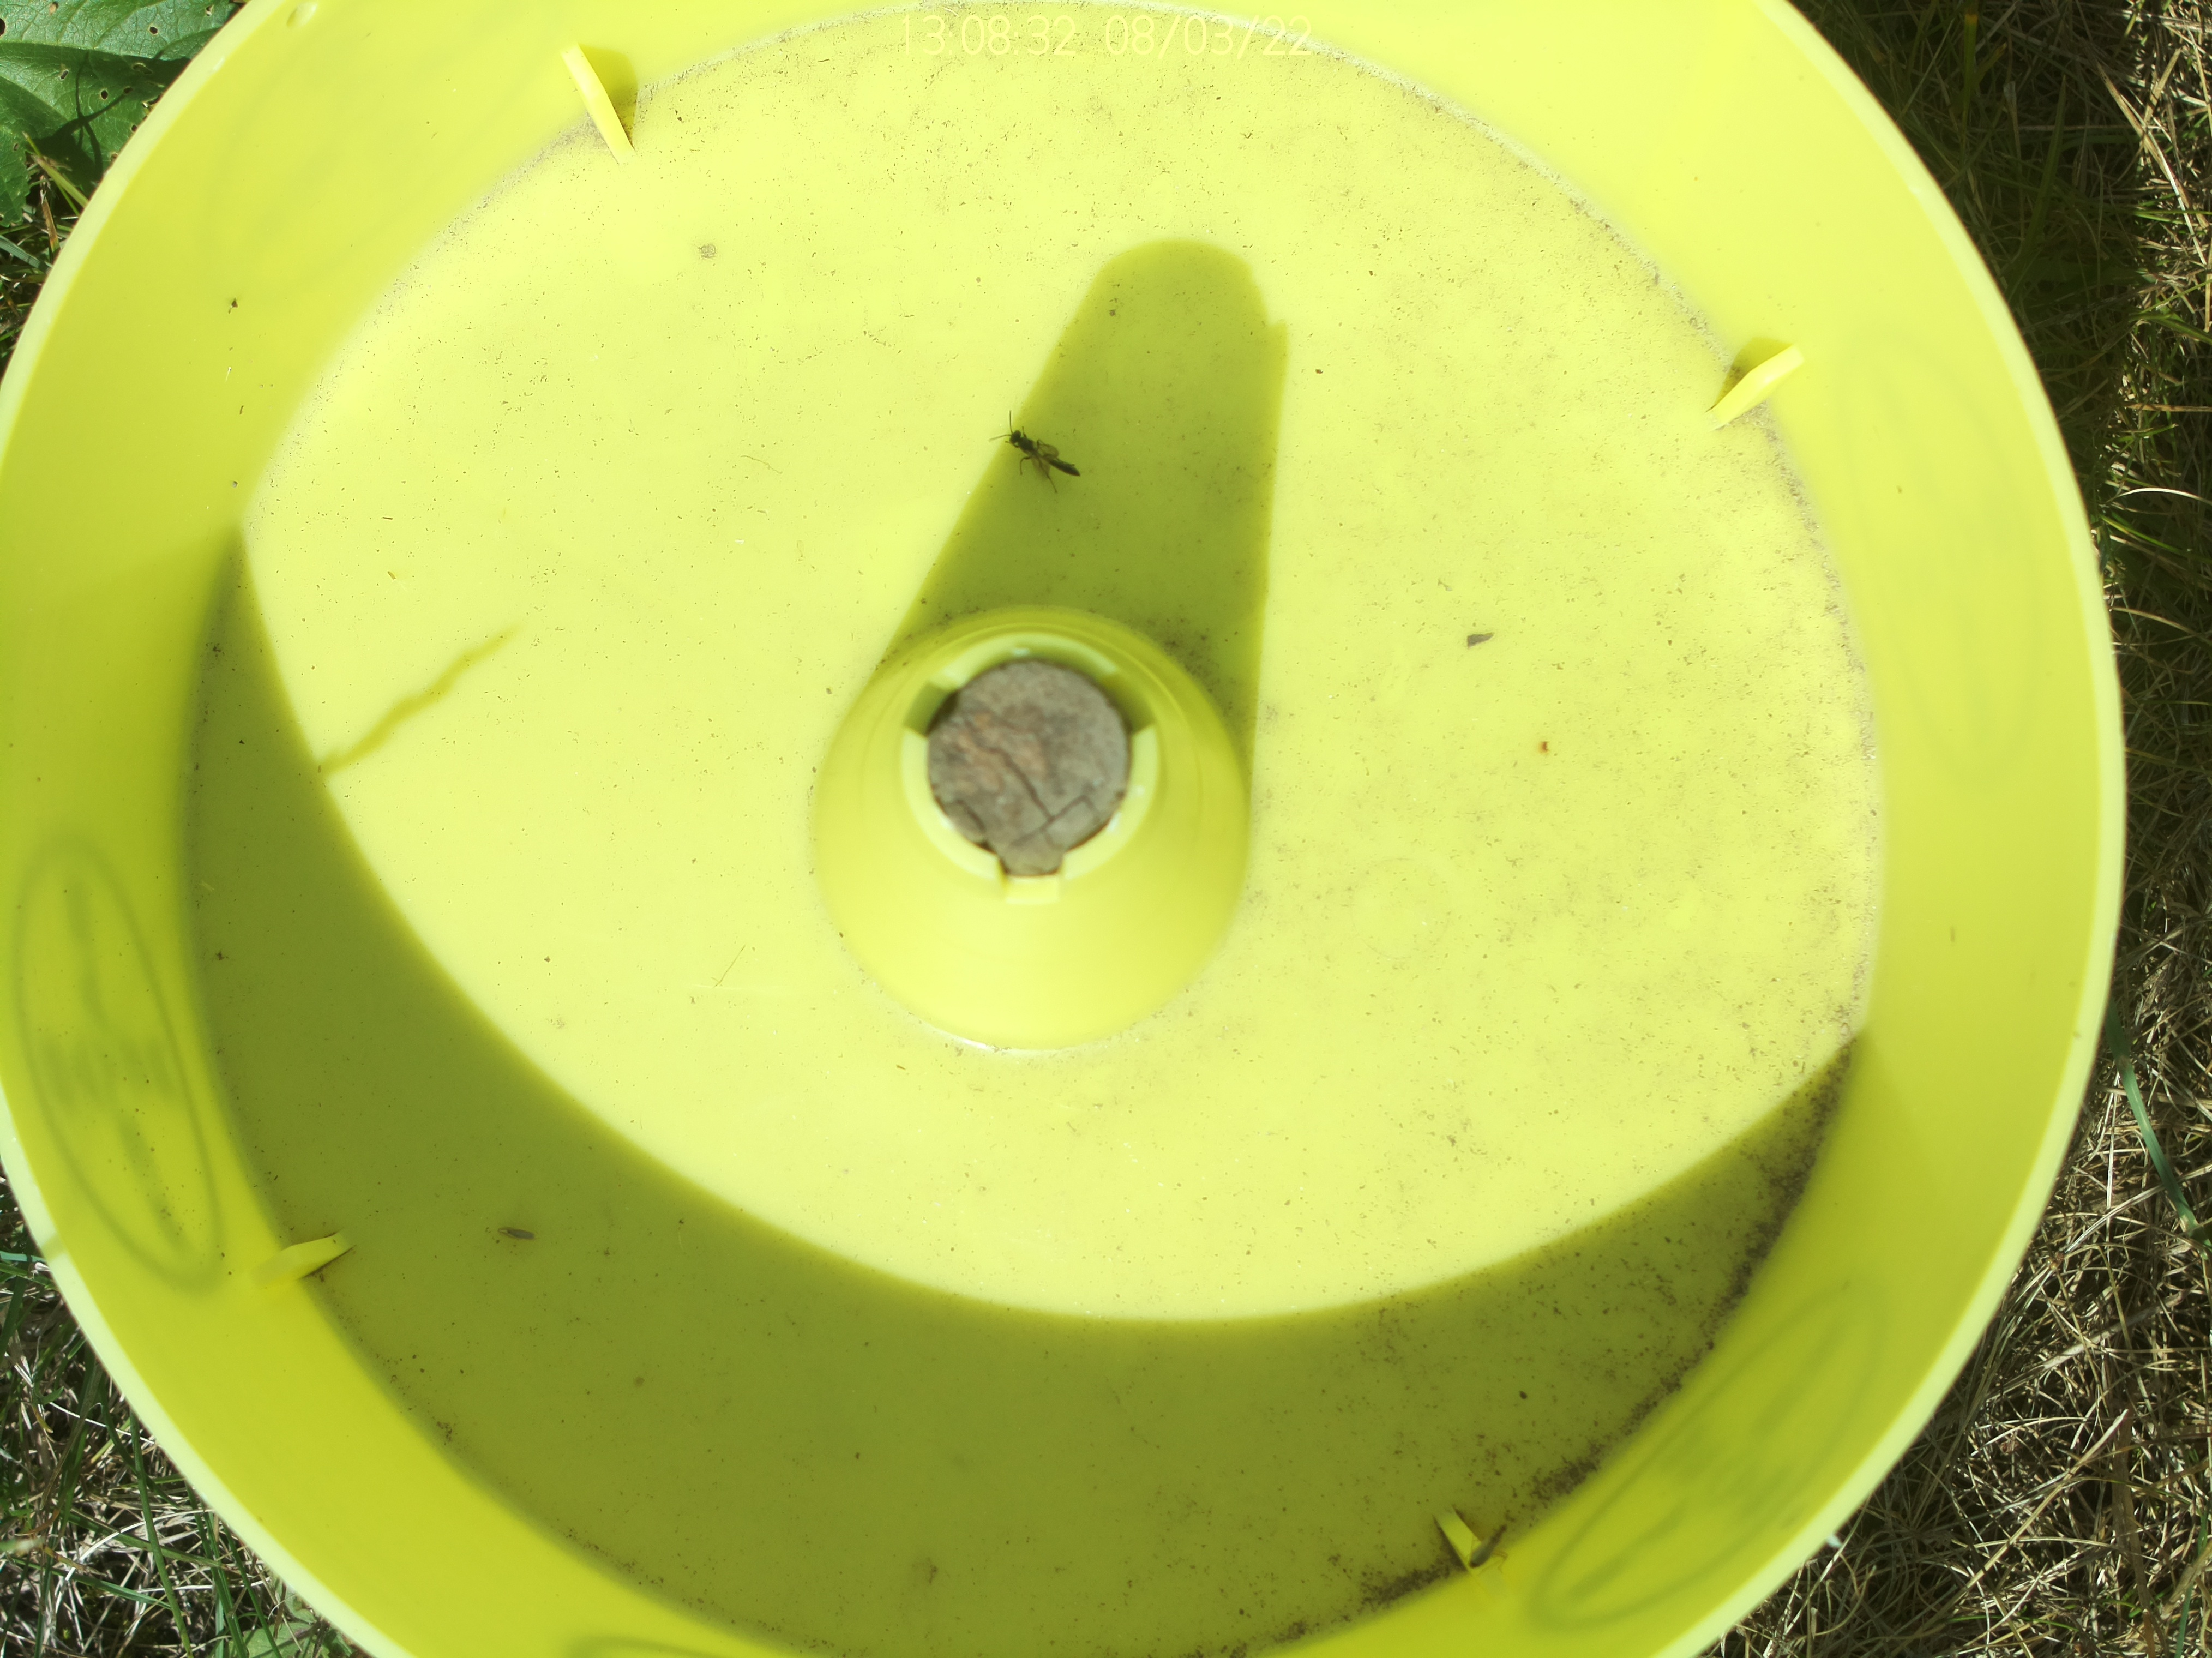
\includegraphics[width=0.5\textwidth]{diff4111}

Das obrige Bild zeigt eine mittelgroße Schwebefliege\\

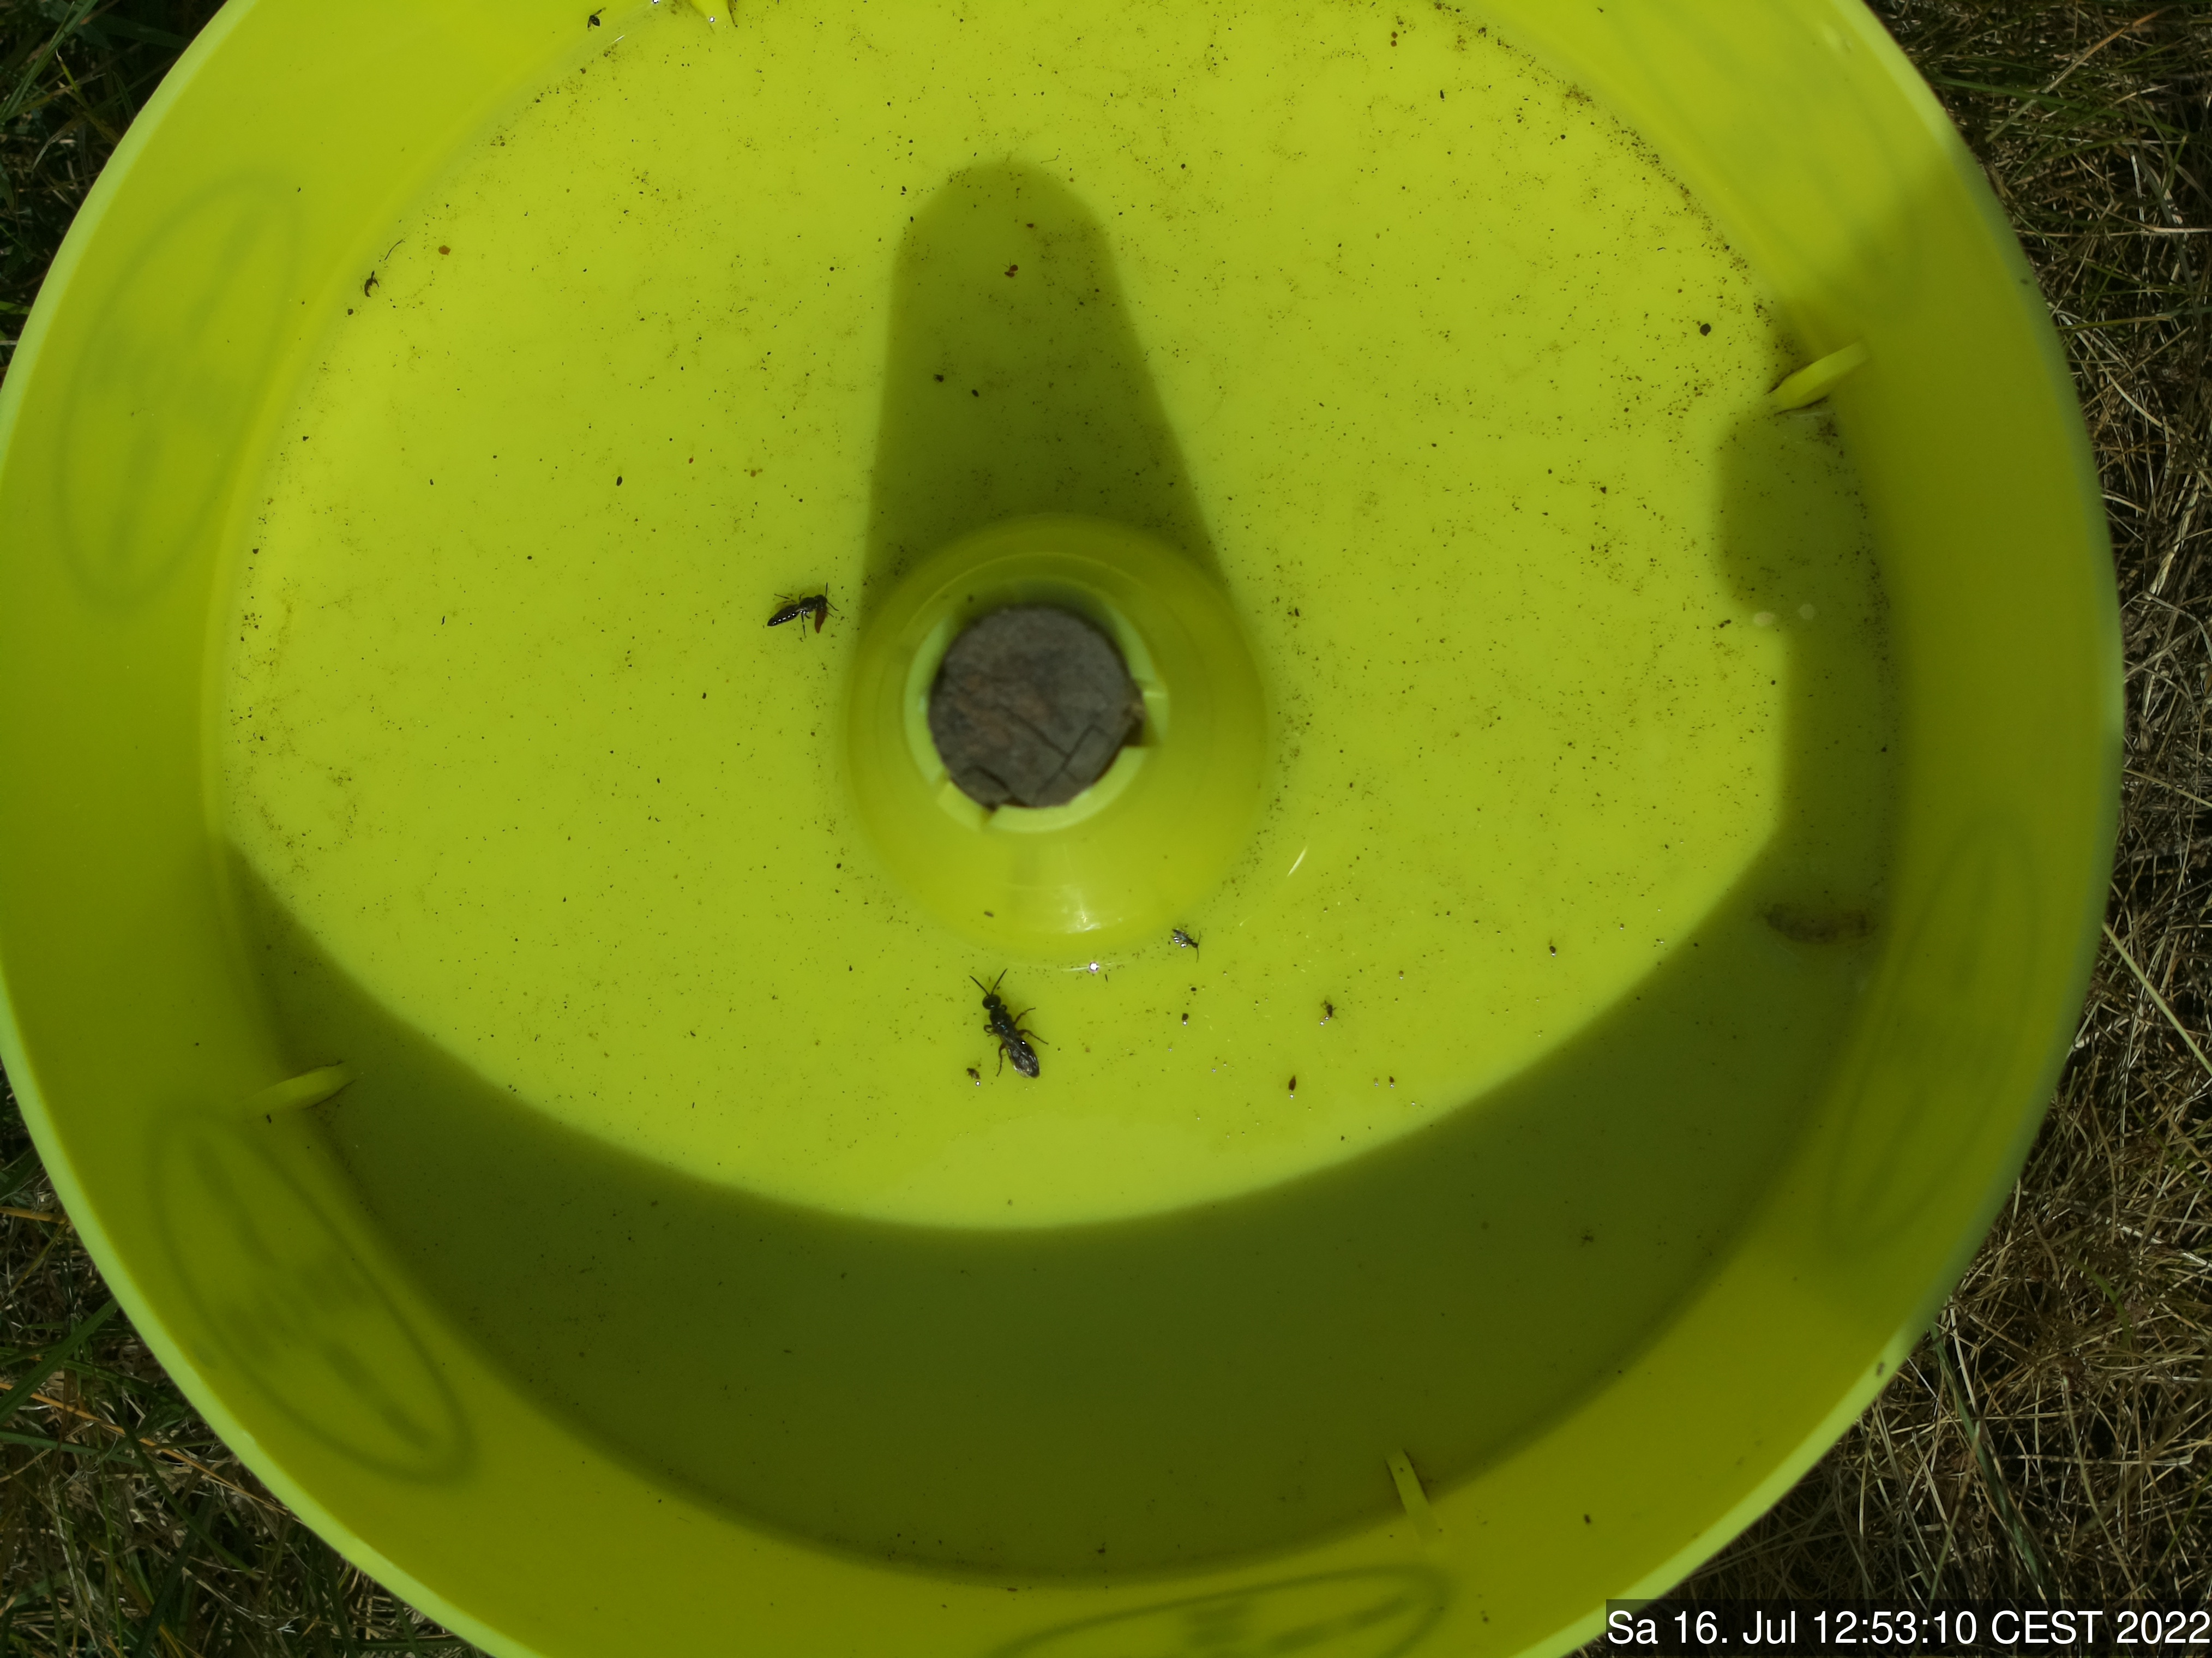
\includegraphics[width=0.5\textwidth]{diff4905}

Das obrige Bild zeigt eine große Schwebefliege\\

\subsection{Labeling}

Zum Laben wurde Roboflow benutzt. Roboflow ist eine eigene Label Software von und für Yolov5. Mit ihr können die Labels in verschiedene
für Yolov5 geeignete Formate exportiert werden.
Der erste benutzte Datensatz beinhaltet 2017 Bilder. 1371 Labels mit dem Titel "Schwebefliege" und 1094 Labels mit dem Titel "Keine Schwebefliege"
wurden gesetzt. Der Datensatz wurde nicht per Augmentation künstlich vergrößert, da Yolo das zum Teil selber macht. Die Verteilung der Insekten auf den Bildern sieht wie folgt aus:\\

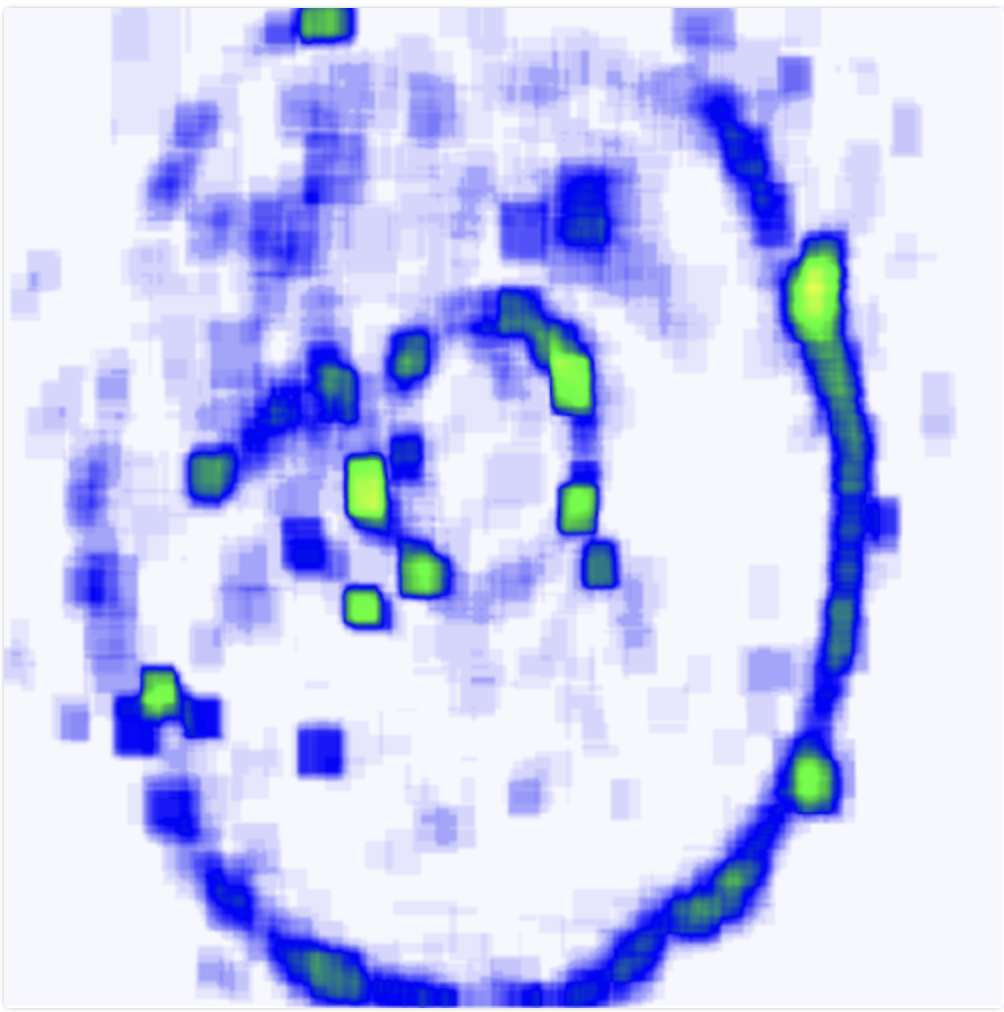
\includegraphics[width=0.5\textwidth]{verteilung}

\subsection{Yolov5 Ausführung}

Das erste Training mit Yolov5 auf diesem Datensatz erfolgte mit default Parametern. (Gewichtung, Bild resizing, epochs)
Über die Software Comet wurden die Ergebnisse in Graphen festgehalten:\\

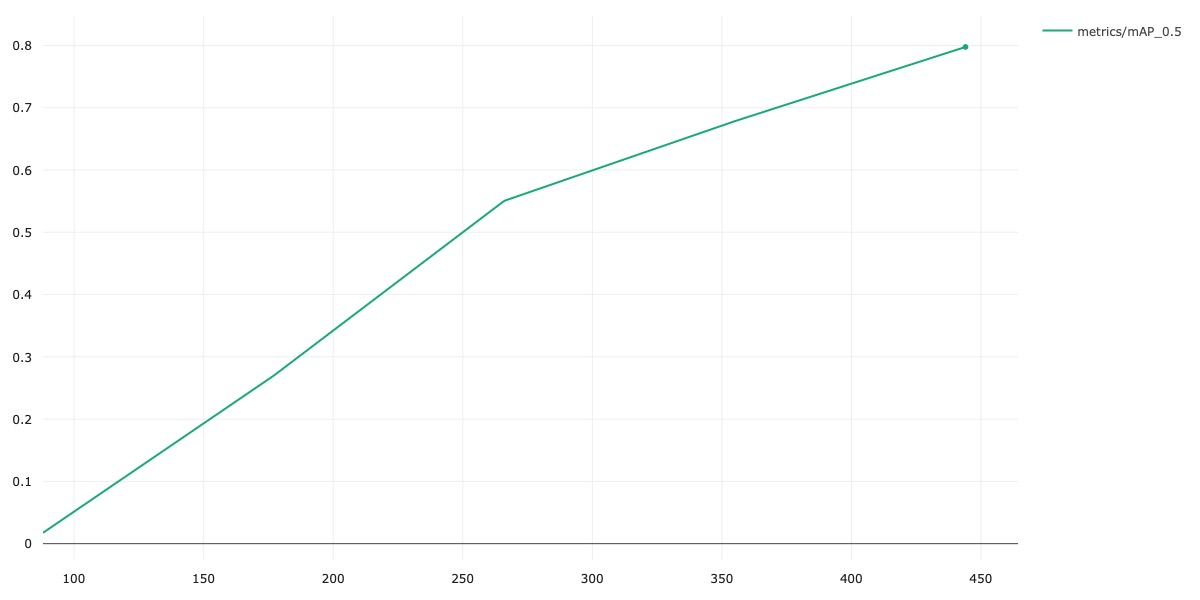
\includegraphics[width=0.5\textwidth]{mAP}\\ Das obrige Bild zeigt den mAP\\

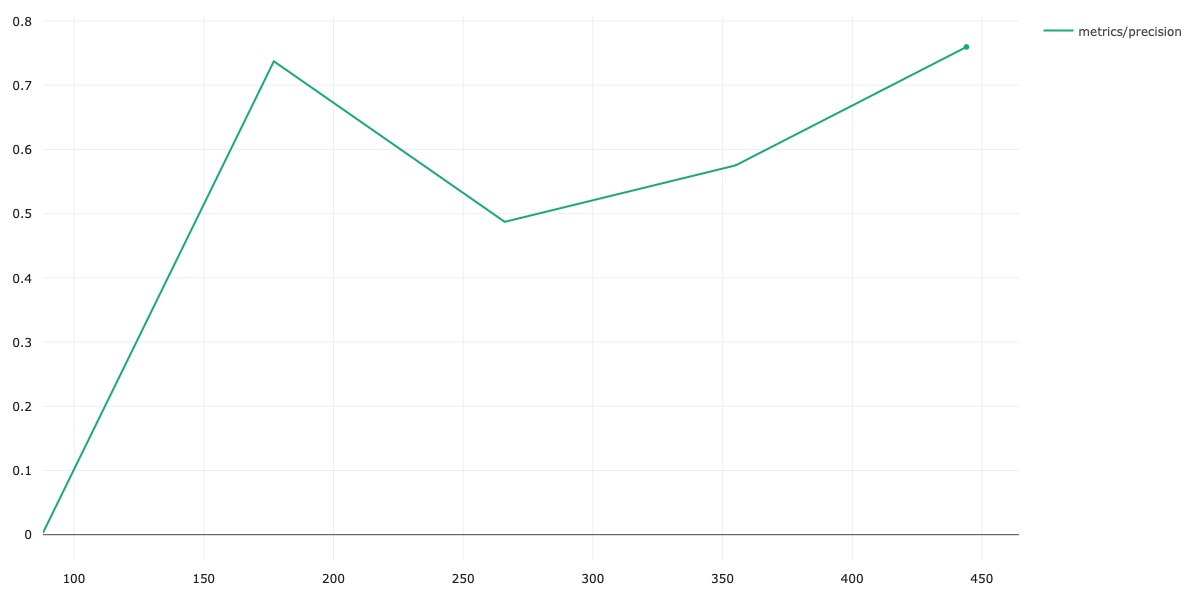
\includegraphics[width=0.5\textwidth]{precision}\\ Das obrige Bild zeigt die Precision\\

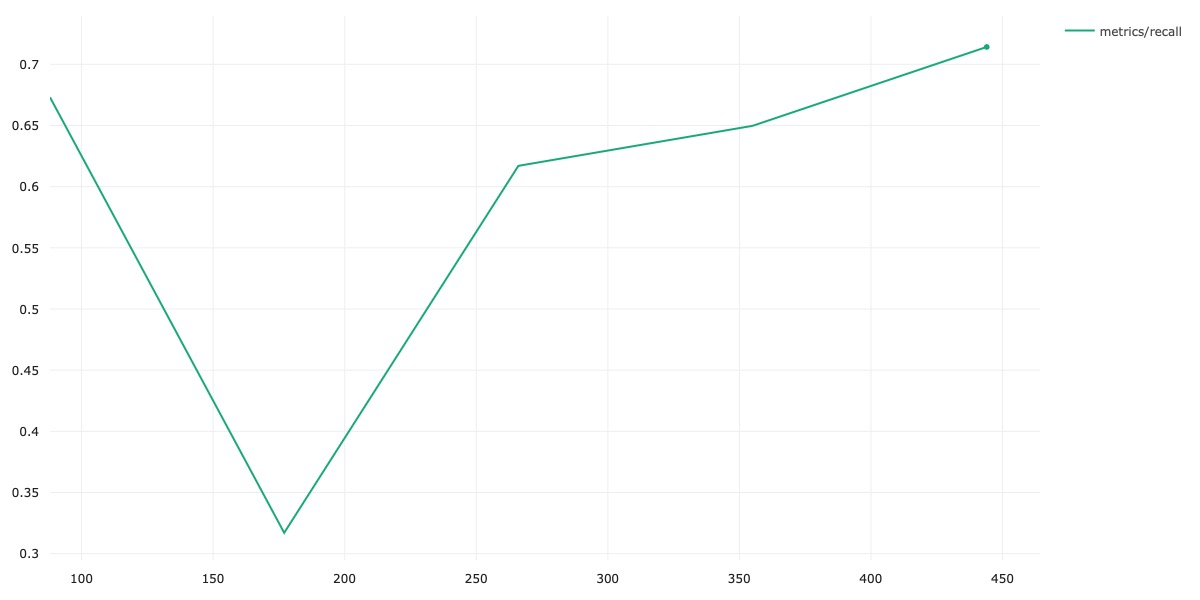
\includegraphics[width=0.5\textwidth]{recall} \\Das obrige Bild zeigt den Recall\\

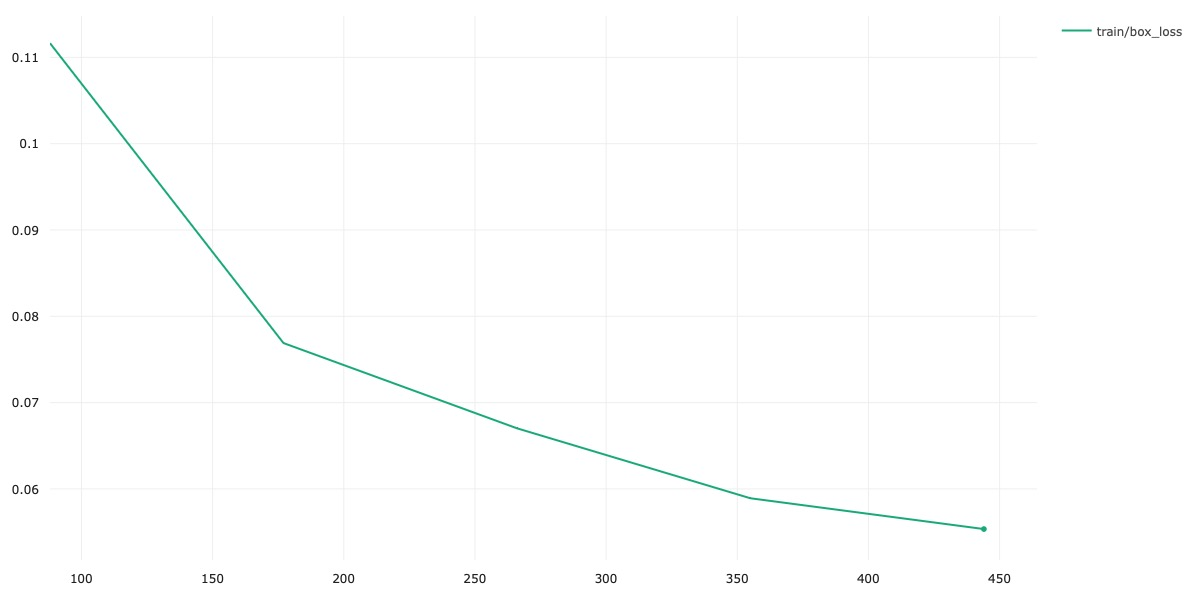
\includegraphics[width=0.5\textwidth]{box_loss}\\ Das obrige Bild zeigt die Regression Box Loss\\

\section{OpenCV vs Yolov5}

\subsection{OpenCV}
Mein object detection Programm verwendet OpenCV ist in 4 Unterprogamme aufgeteilt.
\begin{enumerate}
    \item Differenz Wert \\
    Dieses Programm läuft über den ganzen ungefilterten Bilderordner. Es vergleicht jeweils zwei zeitlich nebeneinander liegende Bilder.
    Diese beiden Bilder werden in die OpenCV absdiff() Funktion gegeben. Die absdiff Funktion berechnet die Differenz zwischen zwei Arrays
    (In OpenCV werden Bilder als Arrays dargestellt). Wenn also der Differenz Wert sehr hoch ist, ist eine bemerkbare Veränderung aufgetreten.
    Die Differenz wurde vorher durch verschiedene Tests von mir festgelegt. Diese Tests wurden an verschiedenen kleineren Datenmengen ausgeführt.
    Die Datenmengen bestanden aus: Einer Testmenge in der nur Bilder sind auf denen sich etwas ändert, eine Testmenge mit Bildern auf denen sich gar nichts ändert,
    und eine Testmenge wo sich ab und an leicht was ändert. Anhand dieser Tests wurde ein fester Differenzwert festgelegt.
    Wenn diesr Differenzwert überschritten wird, wird das erste zu vergleichende Bild in einem neuen Ordner abgespeichert 
    und als Vergleichsbild für das nächste benutzt. Die gefilterten Bilder werden nach ihrem ursprünglichen Ordner und Namen benannt,
    um später wenn nötig das Original wieder zu finden.
    \item Save Originals \\
    Dieses Programm läuft durch den neuen Ordner in dem die Differenzbilder sind und erstellt einen neuen Ordner,
    in dem die dazugehörigen Original Bilder sind. (Die Differenzbilder sind abgedunkelt und heben nur die Stellen hervor, wo etwas passiert)
    Da ja später ein Mensch nochmal über die Bilder drübergucken soll, müssen wir also die dazugehörigen Originale abspeichern.
    \item Cut \\
    Das Cut Programm arbeitet nur auf den Differenzbildern. Es wurde auch getestet, das Programm auf den Originalbildern arbeiten zu
    lassen, die Ergebnisse aus den Tests waren jedoch nicht funktional. Dazu aber später mehr. Da das Programm auf den Differenz Bildern
    arbeitet und die Stellen, die von Interesse sind gehighlited sind muss es zuerst den Rand ignorieren, wie zB das Gras und den Timestamp.
    Dazu wurde eine Maske gefertigt, die nur die Schale hervorhebt. Diese wurde vom Differenzbild abgezogen, jetzt gibt es also nur noch die Schale.
    OpenCV stellt einige Bild Filer Funktionen zur Verfügung. Die besten für diese Aufgabe waren: Gaussian Blur (stellt eine Unschärfe ein),
    ConvertToGray (Grayscale Version des Bildes), convertScaleAbs (lässt einen die Helligkeit anpassen), threshold (findet die hellsten Punkte). Zuerst müssen die Bilder aber
    in zwei Unterkategorien aufgeteilt werden: hell und dunkel. Da die Differenz Bilder jede Veränderung abspeichern, und die Schale draußen stand,
    gibt es durch Wind und Schatten viele Lichtunterschiede. Um diese beiden Arten von Bilder trotzdem gleichermaßen bearbeiten zu können,
    wurde der mean Wert der gesamten Helligkeit berechnet und als Wert benutzt die Bilder zu differnzieren. Wenn ein Bild also zu dunkel ist, wird der
    Helligkeitswert angepasst. Durch die obengenannten Filter werden jetzt alle hellsten Punkte die sich abheben markiert.
    Es entseht ein schwarz-weiß Bild (schwarz der Hintergrund, weiß alles was von Interesse sein könnte). Da hier aber durch die vielen verschiedenen Lichtverhältnisse
    immernoch Regionen vorgehoben werden, die zu groß sind um Insekten zu sein, gibt es festgelegte min und max Werte, die ein Punkt erfüllen
    muss um als interessant kategorisiert zu werden. Von diesen Regionen werden die Kontouren genommen und die Koordinaten abgespeichert, in
    einem separaten Ordner. In diesem existiert für jedes Bild eine txt Datei (damit wir später den Datensatz automatisch erstellen können mit dem wir
    den Algorithmus trainieren) in der der Name des Originalbildes steht und die gefundenen Bounding Box Informationen. Zusätzlich 
    werden die Bounding Boxes ausgeschnitten, man hat also nur noch ein Bild wo nur ein Objekt drauf zu sehen ist. Da die Bounding Box
    Koordinaten sehr genau sind, und die ausgeschnittenen Bilder zu klein für das menschliche Auge sind, gibt es zusätzlich eine Funktion,
    die die Koordinaten der Box vergößert. Diese Funktion muss auch überprüfen ob die jetzt größere Box, zu groß ist, also Koordinaten
    enthält, die gar nicht mehr auf dem ursprünglichen Bild liegen. Fals das der Fall ist, setzt die Funktion die überlaufenden Punkte auf den Rand
    des Original Bildes.
    Noch einmal zum Filtern der Originalbilder; es gibt weitere von OpenCV bereitgestellte Filter Funktionen, die hier auch nochmal zusätzlich
    zu den oben genannten angewand wurden. Die Grundlage der Filter bieten eigentlich immer der gaussian blur und das grayscale image. 
    In Kombination damit wurden die Original Bilder noch mit bilateralFilter(Objekte sind zu klein und ungenau hier um einen guten Effekt zu erzielen,
    dilation (macht die kanten härter und größer, bringt hier aber nichts, da der blur und das grayscale nicht genug ausrichten können),
    erode( macht die kanten weicher und kleiner, entsorgt aber damit auch alle möglichen interessanten Punkte).
    Daher sollte das Programm auf dem Ordner der Differenzbilder arbeiten, anstatt der Originalbilder.
    Zusammenfassend findet das Programm, das auf den Differenzbildern arbeitet mehr als Objekte, aufgrund der verschiedenen Lichtverhältnisse
    werden, trotz filtern, trotzdem noch Bilder gefunden auf denen kein Insekt zu sehen ist. Dies könnte ein Schwerpunkt werden im Vergleich später
    zu Yolo.
    \item Cluster \\
    Es gibt wenige Möglichkeiten die gefundenen Bilder ohne machine learning zu clustern. Die gängiste Methode ist aus den Bildern Histogramme zu erstellen und diese
    dann zu vergleichen. Ein Histogramm aus einem Bild enthält die verschiedenen Farbwerte die darauf zu finden sind. Das Programm vergleicht immer ein Bild mit den restlichen Bildern
    im Ordner. Bilder die gleich sind, werden erstmal in einem Dictionary abgespeichert. Das Programm hat eine Funktion, welche überprüft ob ein Bild
    schon einem Cluster in diesem Dictionary zugeordnet wurde. Wenn das Bild das als Vergleichswert dient noch keinen Dictionary Eintrag hat, wir ein neues
    Cluster erstellt mit diesem Bild als Vergleichswert. Dann werden damit alle folgenden Bilder verglichen. Aus den Bildern werden die Histogramme entnommen
    und per compareHist Funktion wird ein Wert gezogen. Dieser Wert wird überprüft. Wenn er hoch genug ist, werden die Bilder für ähnlich
    befunden und in dasselbe Cluster gepackt. Tests:
    Compare Value: 0.2
    Cluster:
    Read Folder: Small
\end{enumerate}

\subsection{Yolov5}

\begin{enumerate}
    \item da
    
\end{enumerate}


\end{document}
